%!TEX root=kdd15_workshop_main.tex

Distributed, irregular algorithms such as large-scale graph mining nearly always encounter bottlenecks in network communication and load imbalance~\cite{challenglums}. A common preprocessing step is thus mapping this data to processes in a way that alleviates these issues. Graph partitioning is the general problem of dividing a graph into separate components with desired properties; in distributed computing the desired objective is generally equally-sized partitions (to favor load balance) and the minimization of inter-partition edges (to minimize communication).

Formally, we wish to partition the nodes of a graph into $k$ balanced components with capacity $(1+\epsilon)\frac{N}{k}$, such that the number of edges crossing partition boundaries is minimized. Partitioning with these two requirements can be reduced to the minimum-bisection problem~\cite{Garey:1979:CIG:578533} and is therefore NP-Complete. Thus, computing an optimal mapping is generally computationally infeasible, and heuristic approaches are taken. 

\section{Introduction}
\subsection{Graph Partitioning}
\begin{figure}[ht]
\centering
  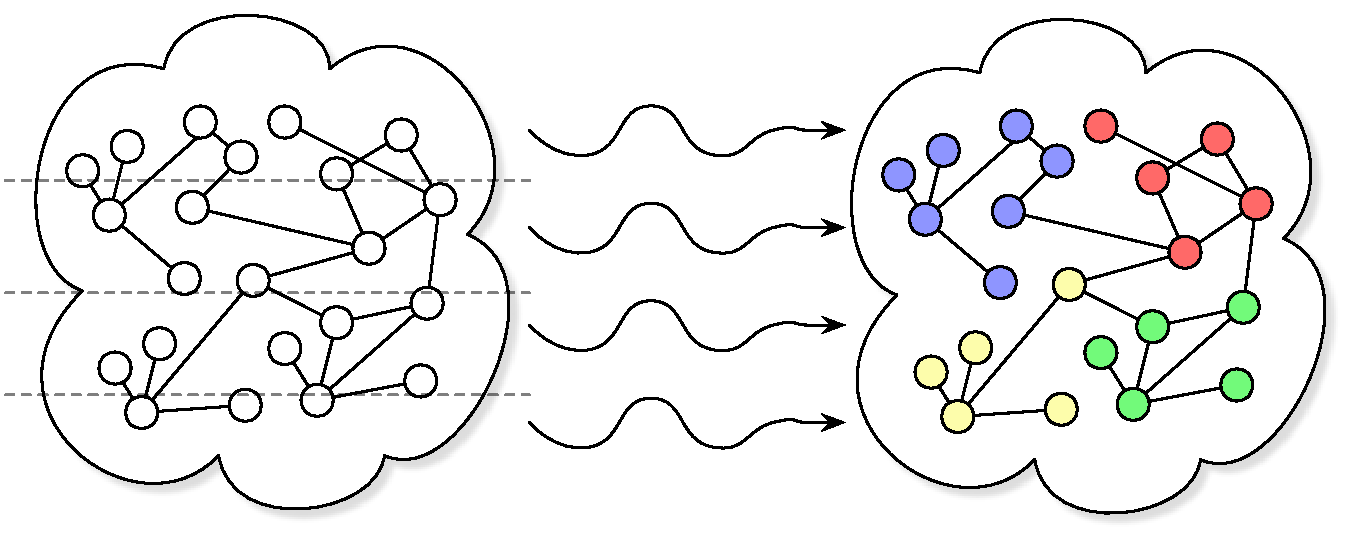
\includegraphics[width=0.7\columnwidth]{figures/coverfig.pdf}
  %\caption{Partition speed of various Kronecker graphs.}
  \label{fig:coverfig}
  \caption{Parallel streaming partitioning.}
\end{figure}

% scenario
To illustrate the role of partitioning on performance, consider a parallel Breadth-First Search (BFS) where a graph's vertices are partitioned between two machines in a `1D' distribution~\cite{Buluc2D}. During each BFS step, each process must communicate all newly explored target vertices to process that owns them. In Figure~\ref{fig:0}, if we have 4 processes, all 14 nonzeros in the non-diagonal blocks must be communicated at some point.
A good partitioner concentrates nonzeros in the diagonal blocks, thereby reducing communication.

Offline graph partitioning algorithms have existed for decades. They work by storing the graph in memory with complete information about the edges. Many variants of these algorithms exist~\cite{gpsurvey} and range from spatial methods~\cite{Gilbert95geometricmesh} to spectral methods~\cite{arora2009expander}. Some of the most effective offline graph partitioners are multi-level partitioners, which recursively contract the graph to a small number of vertices, and then heuristically optimize the partitioning while expanding back to the original graph~\cite{karypis1998multilevel}. Parallel multi-level partitioners will serve as the baseline comparison for our implementation. 

\paragraph{Why Use Streaming Partitioning?}
The most salient property of streaming partitioning is its speed: it can partition the graph in a single sweep, with $O(|V| + |E|)$ memory access, storage, and run time. Existing graph partitioners require the whole graph to be represented in memory, whereas streaming graph partitioning can process vertices as they arrive. This fits a model where input data arrive sequentially from a generating source (such as a web-crawler).

For example, partitioning a 26GB Twitter graph has been shown to take 8 hours using the fastest offline algorithms, and only 40 minutes with the FENNEL partitioner, with similar partition quality~\cite{tsourakakis2012fennel}. This also suggests that we could do multiple, iterative passes of a streaming partitioner, all in a fraction of the time that an offline partitioner would take to terminate~\cite{nishimura2013restream}.

\begin{figure}[h]
\centering
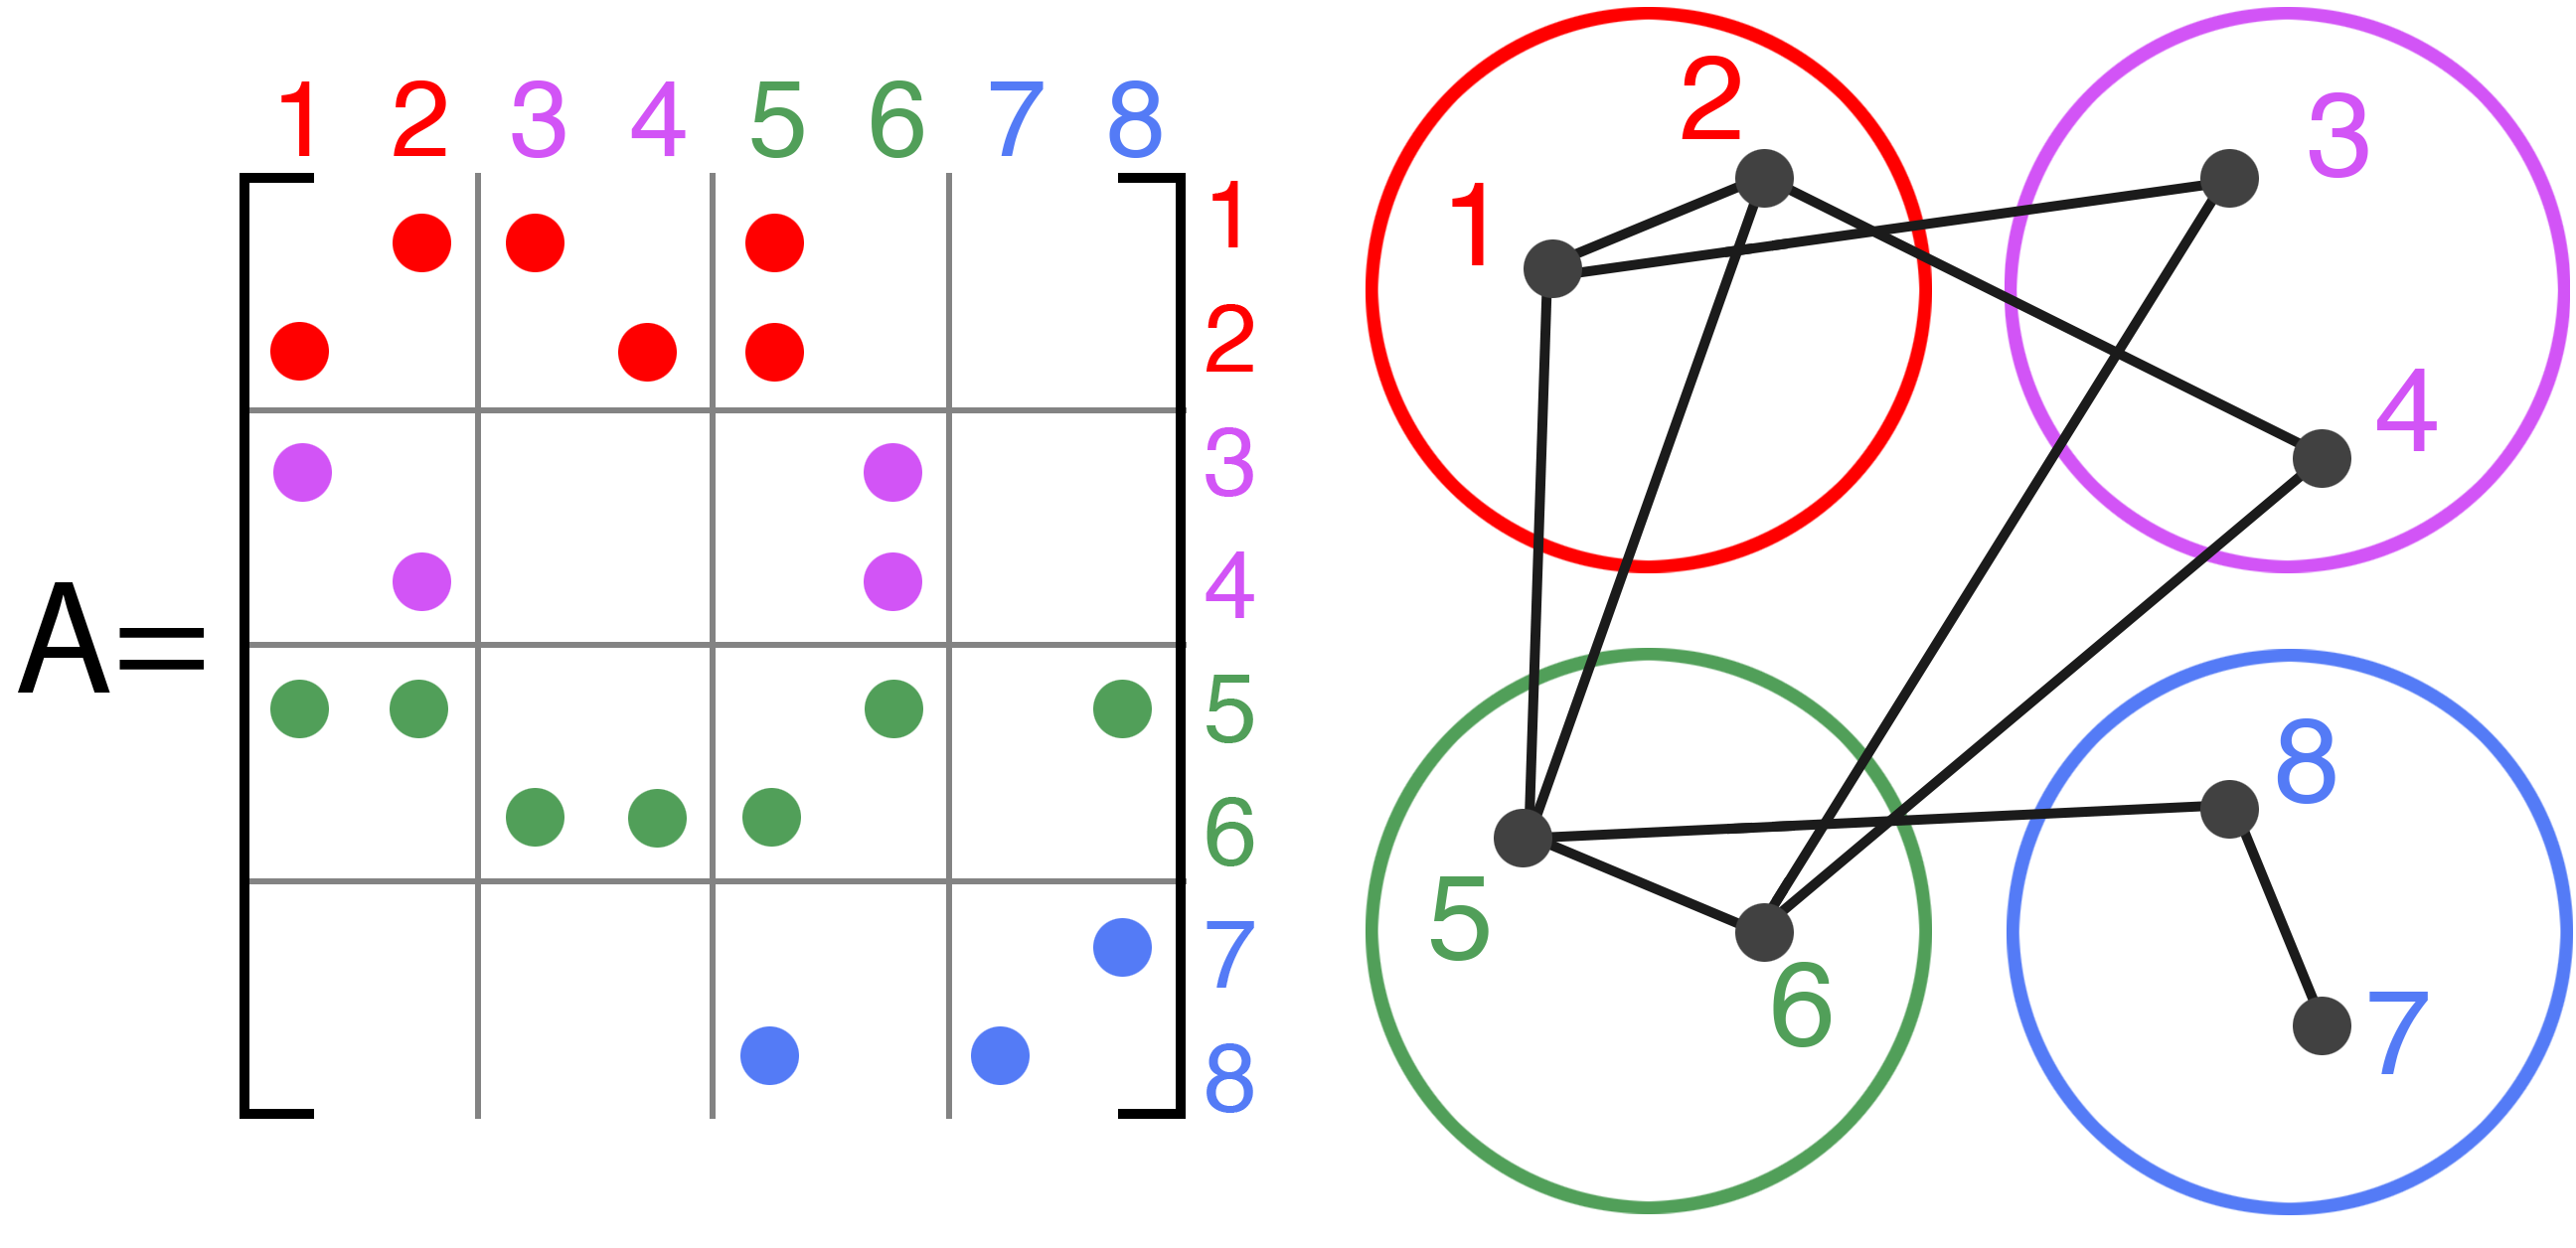
\includegraphics[width=0.85\columnwidth] {figures/graphpart1.png}
\caption[Caption for]{Graph 4-partition shown with corresponding adjacency matrix}
\label{fig:0}
\end{figure}

Streaming partitioning is dependent on the order in which vertices arrive-- commonly in either random order or a breadth-first sequence. An analysis of streaming algorithms may also consider an adversarial ordering that produces the worst possible results~\cite{Stanton:2012:SGP:2339530.2339722}.

We have developed \ourmethod, a fast, iterative, distributed streaming graph partitioner.
It works by restreaming the graph with tempered partition parameters to achieve a fast, parallel \textit{k}-partitioning.
We make the following contributions:
\begin{itemize}
\item A \textbf{scalable} distributed partitioner implementation using MPI.
\item Support for \textbf{streaming} partitioning regardless of stream order.
\item An \textbf{iterative} approach that creates quality partitions.
\end{itemize}



